\chapter{Corchetes de Poisson, generadores y momento angular}

\lectureoverview{El corchete de Poisson es mucho más que una forma compacta de reescribir las ecuaciones de Hamilton. Es una operación algebraica que genera transformaciones. El corchete con el hamiltoniano genera la evolución temporal; con el momento, las traslaciones; y con el momento angular, las rotaciones. En este lenguaje, la simetría y la conservación son dos interpretaciones de un mismo corchete nulo. Desarrollaremos esta idea a partir del oscilador armónico y después usaremos el álgebra del momento angular para obtener la precesión giroscópica sin introducir ángulos de Euler.}

\section{Una función a lo largo de una trayectoria hamiltoniana}

Sea
\[
  F=F(q_1,\ldots,q_n,p_1,\ldots,p_n)
\]
una función suficientemente diferenciable en el espacio de fases. Puede interpretarse de dos maneras. En primer lugar, asigna un número a cada punto del espacio de fases. En segundo lugar, una vez elegida una trayectoria hamiltoniana, se convierte en una función del tiempo porque el punto \((q(t),p(t))\) se mueve. A lo largo de esa trayectoria,
\begin{equation}
  \frac{dF}{dt}
  =
  \sum_i\left(
    \frac{\partial F}{\partial q_i}\dot q_i
    +\frac{\partial F}{\partial p_i}\dot p_i
  \right).
  \label{eq:l8-chain-rule}
\end{equation}
las ecuaciones de Hamilton,
\begin{equation}
  \dot q_i=\frac{\partial H}{\partial p_i},
  \qquad
  \dot p_i=-\frac{\partial H}{\partial q_i},
  \label{eq:l8-hamilton-equations}
\end{equation}
la convierten en
\begin{equation}
  \frac{dF}{dt}
  =
  \sum_i\left(
    \frac{\partial F}{\partial q_i}
    \frac{\partial H}{\partial p_i}
    -
    \frac{\partial F}{\partial p_i}
    \frac{\partial H}{\partial q_i}
  \right).
  \label{eq:l8-fdot-expanded}
\end{equation}
Esta combinación de la derecha aparece por toda la mecánica clásica, incluso cuando ninguno de sus dos argumentos es el hamiltoniano. Esto motiva la definición
\begin{equation}
  \boxed{
  \{F,G\}
  =
  \sum_i\left(
    \frac{\partial F}{\partial q_i}
    \frac{\partial G}{\partial p_i}
    -
    \frac{\partial F}{\partial p_i}
    \frac{\partial G}{\partial q_i}
  \right).}
  \label{eq:l8-poisson-definition}
\end{equation}
Por tanto, la ecuación~\eqref{eq:l8-fdot-expanded} es
\begin{equation}
  \boxed{\dot F=\{F,H\}.}
  \label{eq:l8-time-generator}
\end{equation}

\begin{classroomqa}
  \audiencequestion{Si se cambia el segundo argumento de \(H\) por una función arbitraria
  \(G\), ¿el corchete sigue siendo la derivada temporal de \(F\)?
  \lecturetimestamp{00:05:45--00:06:15}}
  \lecturerresponse{No. Mientras se generaliza la notación, alguien del público capta un punto importante. La ecuación~\eqref{eq:l8-poisson-definition}
  define \(\{F,G\}\) para cualesquiera dos funciones del espacio de fases, pero
  \(\dot F=\{F,G\}\) solo se cumple cuando \(G\) es el hamiltoniano. Una función
  \(G\) general generará una transformación infinitesimal distinta.}
\end{classroomqa}

Es útil escribir un pequeño intervalo de tiempo como
\begin{equation}
  \delta_t F=\epsilon\,\{F,H\}.
  \label{eq:l8-small-time-step}
\end{equation}
Esta forma anticipa lo que veremos más adelante. La evolución temporal es un elemento de una familia más amplia de transformaciones generadas por corchetes de Poisson.

\section{El álgebra de los corchetes}

Ahora podemos usar el corchete como un cálculo por derecho propio. Sus reglas se deducen de la diferenciación ordinaria:
\begin{align}
  \{A,B\}&=-\{B,A\}, \label{eq:l8-antisymmetry}\\
  \{A+B,C\}&=\{A,C\}+\{B,C\}, \label{eq:l8-additivity}\\
  \{\lambda A,B\}&=\lambda\{A,B\},
    \quad \lambda\ \text{constant}, \label{eq:l8-scalar-rule}\\
  \{AB,C\}&=A\{B,C\}+\{A,C\}B. \label{eq:l8-leibniz}
\end{align}
Estas cuatro líneas expresan, respectivamente, la antisimetría, la aditividad, la linealidad respecto de la multiplicación por una constante y la regla de Leibniz.
Las funciones del espacio de fases clásico se multiplican de forma conmutativa, así que el orden de los factores ordinarios \(A\) y \(B\) en la última línea es irrelevante. Esto dejará de ser cierto para los operadores de la mecánica cuántica. La antisimetría también implica
\begin{equation}
  \{A,A\}=0.
  \label{eq:l8-self-bracket}
\end{equation}

Para las coordenadas canónicas, los corchetes elementales son
\begin{equation}
  \boxed{
  \{q_i,q_j\}=0,\qquad
  \{p_i,p_j\}=0,\qquad
  \{q_i,p_j\}=\delta_{ij}.}
  \label{eq:l8-canonical-brackets}
\end{equation}
Cualquier función que dependa solo de las \(q_i\) tiene corchete nulo con cualquier otra función que dependa solo de las \(q_i\); lo mismo vale para las funciones que dependen solo de los \(p_i\). Para que el corchete sea distinto de cero, una coordenada canónica debe encontrarse con su momento conjugado. La delta de Kronecker en la ec.~\eqref{eq:l8-canonical-brackets} indica que solo se emparejan los índices coincidentes.

\subsection{El oscilador armónico como prueba}

Consideremos
\begin{equation}
  H=\frac{p^2}{2m}+\frac{kq^2}{2}.
  \label{eq:l8-oscillator-hamiltonian}
\end{equation}
Ahora usaremos deliberadamente solo las reglas de los corchetes y la ec.~\eqref{eq:l8-time-generator}. En primer lugar,
\begin{align}
  \dot q
  &=\{q,H\}\\
  &=\frac{1}{2m}\{q,p^2\}\\
  &=\frac{1}{2m}\left(p\{q,p\}+\{q,p\}p\right)\\
  &=\frac{p}{m}.
  \label{eq:l8-qdot-oscillator}
\end{align}
El término de potencial desaparece porque \(\{q,q^2\}=0\). De manera similar,
\begin{align}
  \dot p
  &=\{p,H\}\\
  &=\frac{k}{2}\{p,q^2\}\\
  &=\frac{k}{2}\left(q\{p,q\}+\{p,q\}q\right)\\
  &=-kq.
  \label{eq:l8-pdot-oscillator}
\end{align}
El signo menos se debe precisamente a la antisimetría
\(\{p,q\}=-\{q,p\}=-1\). Al combinar las dos ecuaciones de primer orden se obtiene
\begin{equation}
  m\ddot q=-kq.
  \label{eq:l8-hooke-equation}
\end{equation}

\begin{figure}[htbp]
  \centering
  
\includegraphics[width=0.82\textwidth]{lecture_08_figure_01.png}
  \caption{El hamiltoniano del oscilador y los dos cálculos de corchetes que dan \(\dot q=p/m\) y \(\dot p=-kq\).}
  \lectureframe{00:23:20}
\end{figure}

Durante el cálculo, la clase busca un verbo que signifique
\emph{calcular un corchete de Poisson} y, provisionalmente, propone
\emph{poissonizar}. La broma señala un cambio de perspectiva real: una vez conocido el álgebra, se puede trabajar directamente con ella en vez de volver a derivar cada resultado a partir de la definición.

\begin{classroomqa}
  \audiencequestion{¿Esta estructura matemática es un grupo o un álgebra?
  ¿Tiene inversos? \lecturetimestamp{00:23:48--00:24:16}}
  \lecturerresponse{No es un grupo: la operación de corchete no proporciona la identidad ni los inversos requeridos. Las funciones del espacio de fases forman un álgebra de Poisson: tienen suma y producto conmutativos ordinarios, además de un corchete antisimétrico que cumple la regla de Leibniz. Una identidad adicional, la identidad de Jacobi, completa la definición abstracta habitual, aunque no se desarrolla en esta lección.}
\end{classroomqa}

\begin{classroomqa}
  \audiencequestion{¿Qué relación hay entre los corchetes de Poisson y los conmutadores cuánticos? \lecturetimestamp{00:24:18--00:25:00}}
  \lecturerresponse{La lección solo ofrece un anticipo. En el paso a la mecánica cuántica, el corchete clásico se sustituye esquemáticamente por
  \[
    \{A,B\}_{\mathrm{PB}}
    \longleftrightarrow
    \frac{1}{i\hbar}[\widehat A,\widehat B].
  \]
  Esta correspondencia requiere matices relacionados con el orden de los operadores y la cuantización; aquí no se usa como teorema.}
\end{classroomqa}

Para el oscilador, el corchete no ha hecho más que reconstruir las ecuaciones de Hamilton. Su verdadera utilidad se aprecia cuando el generador es una cantidad conservada distinta de \(H\).

\section{Recuperación del momento angular a partir de la simetría rotacional}

Recordemos la forma infinitesimal de la construcción de Noether que vimos antes en el curso. Si una simetría continua cambia las coordenadas según
\begin{equation}
  \delta q_i=\epsilon F_i(q),
  \label{eq:l8-noether-variation}
\end{equation}
entonces, en el caso que consideramos aquí, la cantidad conservada es
\begin{equation}
  G=\sum_i p_iF_i(q).
  \label{eq:l8-noether-charge}
\end{equation}
Se puede omitir el factor global \(\epsilon\): multiplicar una cantidad conservada por un número fijo no altera la ley de conservación.

Tomemos una partícula y hagámosla rotar infinitesimalmente alrededor del eje \(z\). Con la orientación usada en la lección,
\begin{equation}
  \delta x=-\epsilon y,\qquad
  \delta y=\epsilon x,\qquad
  \delta z=0.
  \label{eq:l8-z-rotation}
\end{equation}
La ecuación~\eqref{eq:l8-noether-charge} da
\begin{equation}
  L_z=-p_xy+p_yx=xp_y-yp_x.
  \label{eq:l8-lz}
\end{equation}
Al hacer permutaciones cíclicas de \(x\), \(y\) y \(z\),
\begin{equation}
  \boxed{\begin{aligned}
    L_x&=yp_z-zp_y,\\
    L_y&=zp_x-xp_z,\\
    L_z&=xp_y-yp_x.
  \end{aligned}}
  \label{eq:l8-angular-components}
\end{equation}
que son las componentes de
\begin{equation}
  \boldsymbol L=\boldsymbol r\times\boldsymbol p.
  \label{eq:l8-cross-product}
\end{equation}

\begin{figure}[htbp]
  \centering
  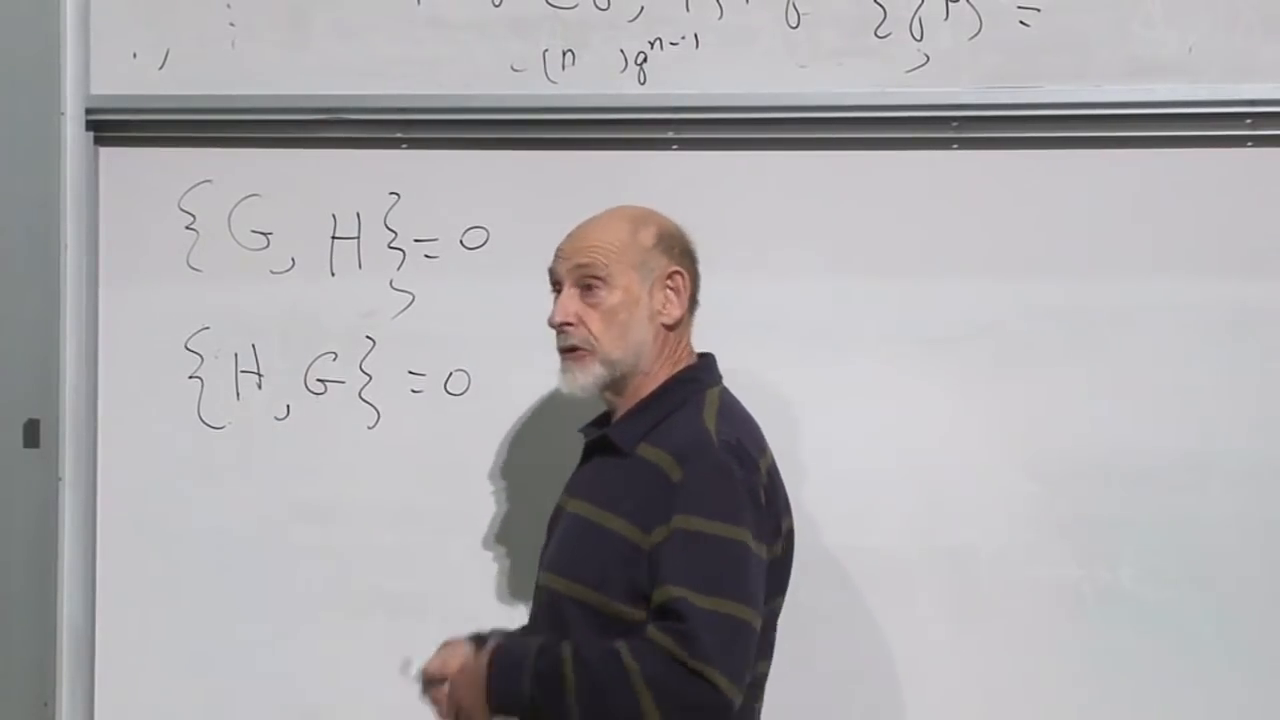
\includegraphics[width=0.82\textwidth]{lecture_08_figure_02.png}
  \caption{Las tres componentes cartesianas del momento angular y su forma compacta mediante el producto vectorial.}
  \lectureframe{00:34:00}
\end{figure}

La rotación alrededor de un vector unitario arbitrario \(\boldsymbol n\) está generada por
\begin{equation}
  L_{\boldsymbol n}=\boldsymbol n\cdot\boldsymbol L.
  \label{eq:l8-arbitrary-axis}
\end{equation}
En un sistema aislado e invariante ante rotaciones, se conservan las tres componentes. Si solo las rotaciones alrededor de un eje siguen siendo simetrías, únicamente se garantiza la conservación de la componente a lo largo de ese eje.

\section{El momento angular genera rotaciones}

En lugar de resolver de inmediato un problema de dinámica rotacional, exploremos qué hace \(L_z\) bajo el corchete. Usando la
ec.~\eqref{eq:l8-lz},
\begin{align}
  \{x,L_z\}
  &=\{x,xp_y-yp_x\}
   =-y\{x,p_x\}
   =-y,\\
  \{y,L_z\}
  &=\{y,xp_y-yp_x\}
   =x\{y,p_y\}
   =x,\\
  \{z,L_z\}&=0.
  \label{eq:l8-position-rotation-brackets}
\end{align}
Estos son exactamente los coeficientes de la ec.~\eqref{eq:l8-z-rotation}.

\begin{figure}[htbp]
  \centering
  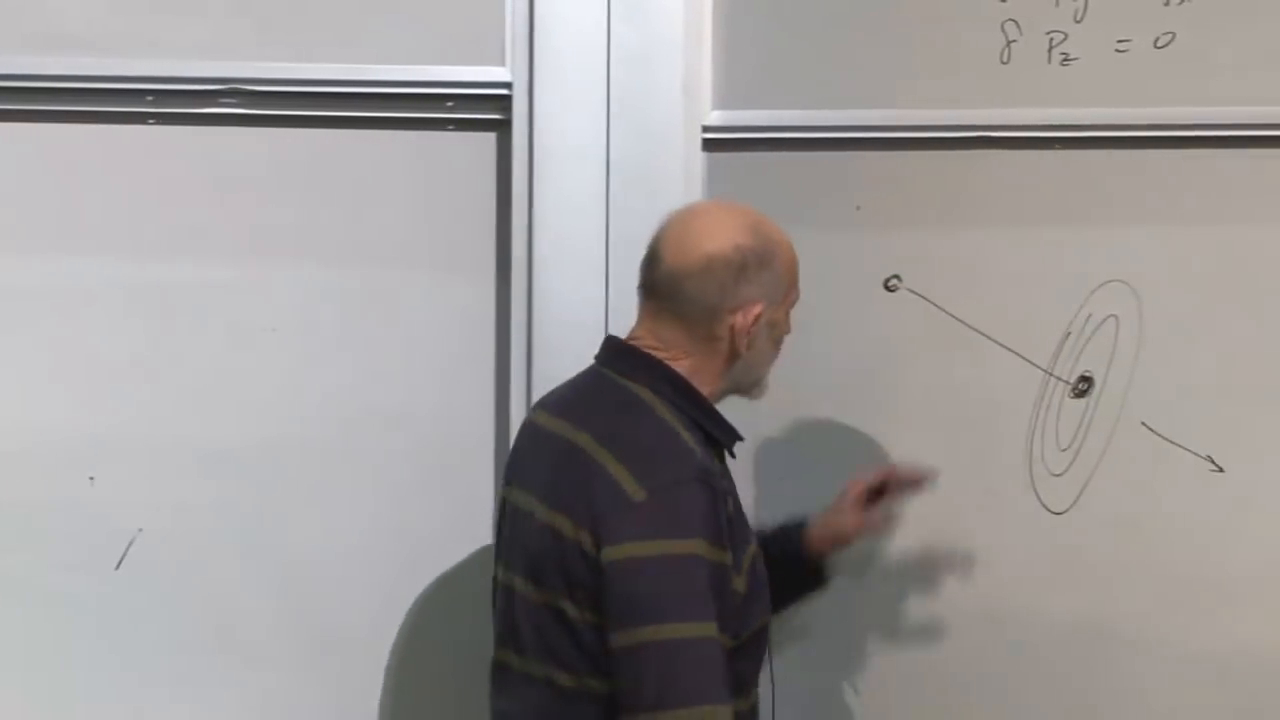
\includegraphics[width=0.82\textwidth]{lecture_08_figure_03.png}
  \caption{Los corchetes de las coordenadas con \(L_z\): el corchete reproduce la rotación infinitesimal de \((x,y,z)\).}
  \lectureframe{00:38:41}
\end{figure}

El momento también es un vector, y el mismo cálculo da
\begin{equation}
  \begin{aligned}
    \{p_x,L_z\}&=-p_y,\\
    \{p_y,L_z\}&=p_x,\\
    \{p_z,L_z\}&=0.
  \end{aligned}
  \label{eq:l8-momentum-rotation-brackets}
\end{equation}

\begin{figure}[htbp]
  \centering
  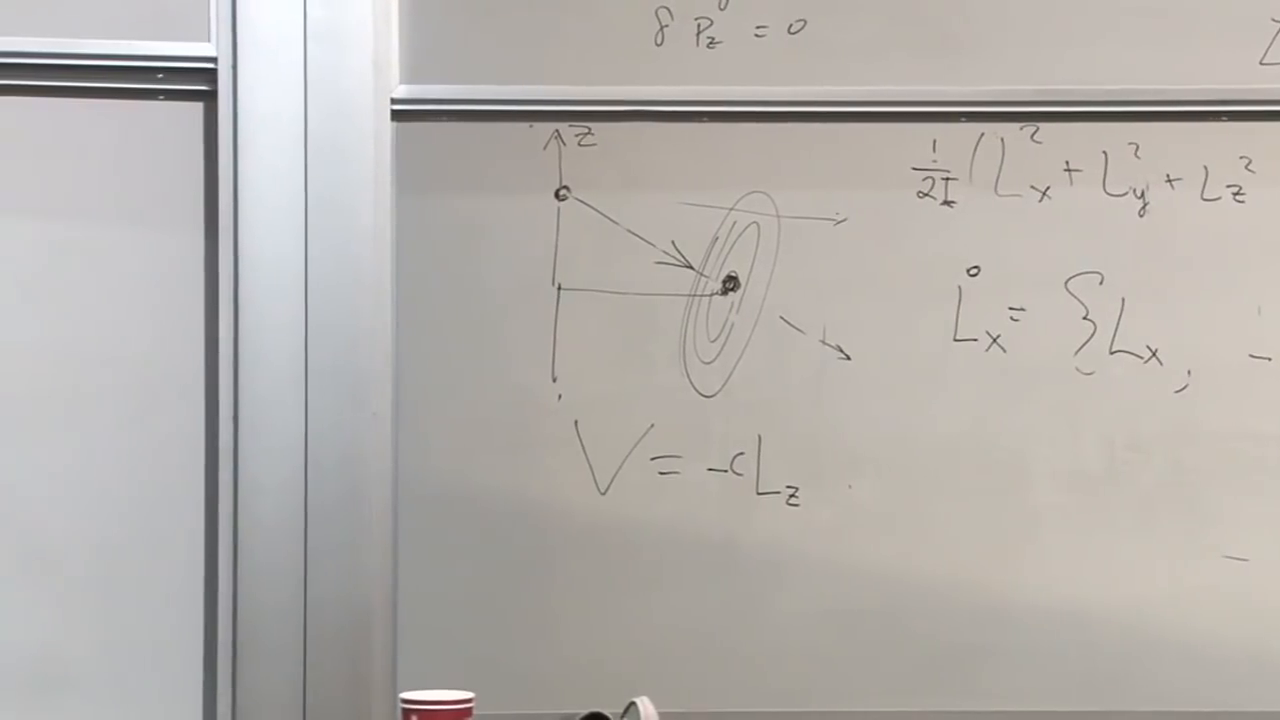
\includegraphics[width=0.82\textwidth]{lecture_08_figure_04.png}
  \caption{La posición y el momento siguen el mismo patrón vectorial bajo la rotación generada por \(L_z\).}
  \lectureframe{00:42:08}
\end{figure}

Por tanto, el enunciado hamiltoniano general es
\begin{equation}
  \boxed{\delta_G A=\epsilon\{A,G\}.}
  \label{eq:l8-generator-rule}
\end{equation}
Toda función del espacio de fases \(G\) define una transformación canónica infinitesimal de este tipo. Si \(G=L_z\), se trata de una rotación. Si \(G=H\), es un pequeño paso en el tiempo.

\begin{classroomqa}
  \audiencequestion{En la lección se habla a veces de rotar el sistema y otras de rotar las coordenadas. ¿Qué convención se usa en las ecuaciones de corchetes? \lecturetimestamp{00:28:22--00:29:35}}
  \lecturerresponse{La ecuación~\eqref{eq:l8-z-rotation} fija la convención: se trata de la rotación activa infinitesimal
  \((x,y)\mapsto(x-\epsilon y,y+\epsilon x)\). Una rotación pasiva de los ejes tiene el signo opuesto. Una vez fijada la convención, las fórmulas de los corchetes no dejan lugar a ambigüedades.}
\end{classroomqa}

\section{El momento genera traslaciones}

Una traslación en una coordenada tiene
\begin{equation}
  \delta q=\epsilon.
  \label{eq:l8-q-translation}
\end{equation}
Aquí \(F(q)=1\) en la ec.~\eqref{eq:l8-noether-variation}, así que la cantidad conservada correspondiente es \(p\). La afirmación sobre el generador predice
\begin{equation}
  \{f(q),p\}=\frac{df}{dq}.
  \label{eq:l8-translation-derivative}
\end{equation}
La lección demuestra primero este resultado para potencias, por inducción. El caso base es
\(\{q,p\}=1\). Supongamos que
\begin{equation}
  \{q^{n-1},p\}=(n-1)q^{n-2}.
  \label{eq:l8-induction-hypothesis}
\end{equation}
Entonces, la regla del producto da
\begin{align}
  \{q^n,p\}
  &=\{q\,q^{n-1},p\}\\
  &=q\{q^{n-1},p\}+\{q,p\}q^{n-1}\\
  &=(n-1)q^{n-1}+q^{n-1}\\
  &=nq^{n-1}.
  \label{eq:l8-power-translation}
\end{align}
La linealidad extiende el resultado a los polinomios y a las representaciones mediante series de potencias convergentes. De forma más directa, la definición del corchete da la ec.~\eqref{eq:l8-translation-derivative} para toda función diferenciable \(f(q)\):
\begin{equation}
  \{f(q),p\}
  =
  \frac{\partial f}{\partial q}
  \frac{\partial p}{\partial p}
  =f'(q).
\end{equation}

\begin{figure}[htbp]
  \centering
  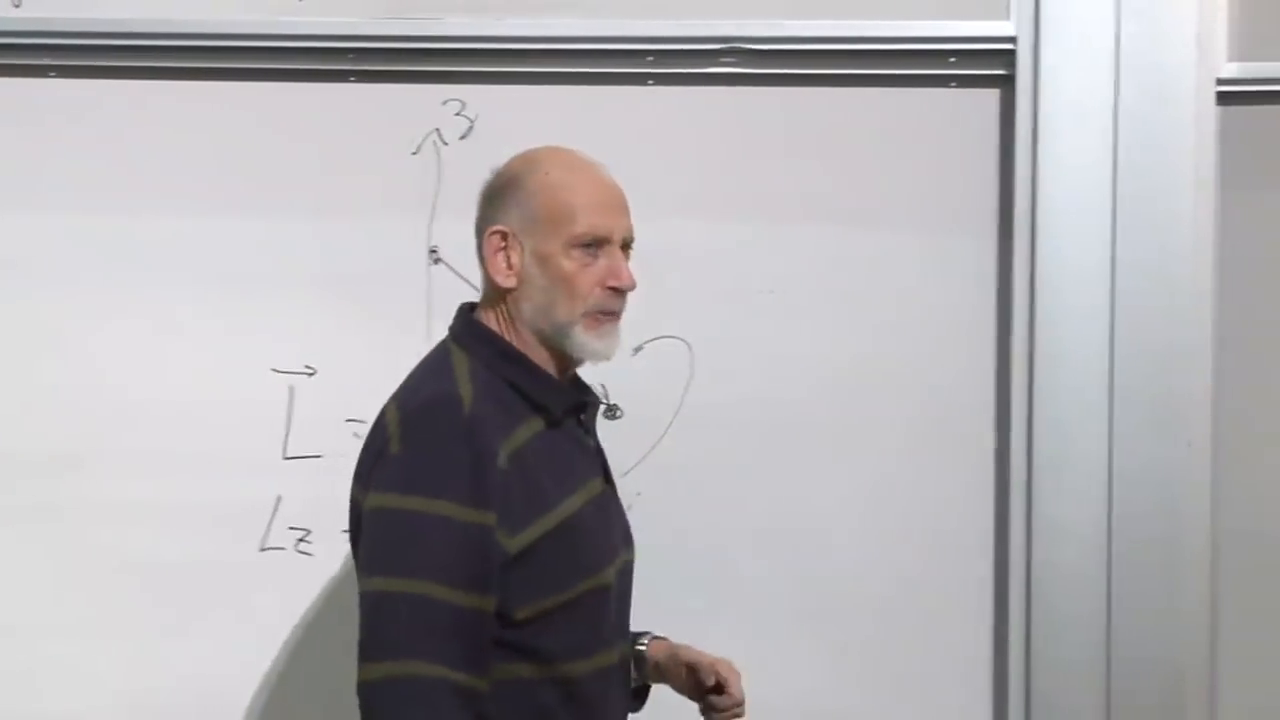
\includegraphics[width=0.82\textwidth]{lecture_08_figure_05.png}
  \caption{El resultado de la traslación tras el argumento por inducción:
  \(\{F(q),p\}=dF/dq\).}
  \lectureframe{00:53:18}
\end{figure}

Hemos visto tres versiones de una misma idea:
\begin{center}
  \begin{tabular}{@{}>{\raggedright\arraybackslash}p{0.37\textwidth}
                      >{\raggedright\arraybackslash}p{0.55\textwidth}@{}}
    \toprule
    Generador y transformación & Acción infinitesimal\\
    \midrule
    \(H\), traslación temporal & \(\delta_tA=\epsilon\{A,H\}\)\\
    \(p_i\), traslación espacial & \(\delta A=\epsilon\{A,p_i\}\)\\
    \(L_i\), rotación & \(\delta A=\epsilon\{A,L_i\}\)\\
    \bottomrule
  \end{tabular}
\end{center}
La cantidad conservada asociada a una simetría continua es también el generador de esa simetría.

\section{Un corchete, dos interpretaciones}

Sea \(G(q,p)\) un posible generador. Si se conserva y no depende explícitamente del tiempo, entonces
\begin{equation}
  \dot G=\{G,H\}=0.
  \label{eq:l8-g-conserved}
\end{equation}
Por antisimetría,
\begin{equation}
  \{H,G\}=0.
  \label{eq:l8-h-invariant}
\end{equation}
Las ecuaciones son matemáticamente equivalentes, pero su interpretación física es distinta:
\begin{itemize}
  \item \(\{G,H\}=0\) indica que \(G\) no cambia durante la evolución temporal generada por \(H\).
  \item \(\{H,G\}=0\) indica que \(H\) no cambia bajo la transformación generada por \(G\).
\end{itemize}
La primera es una ley de conservación; la segunda, una simetría del hamiltoniano. La relación de Noether queda condensada en un cero.

\begin{figure}[htbp]
  \centering
  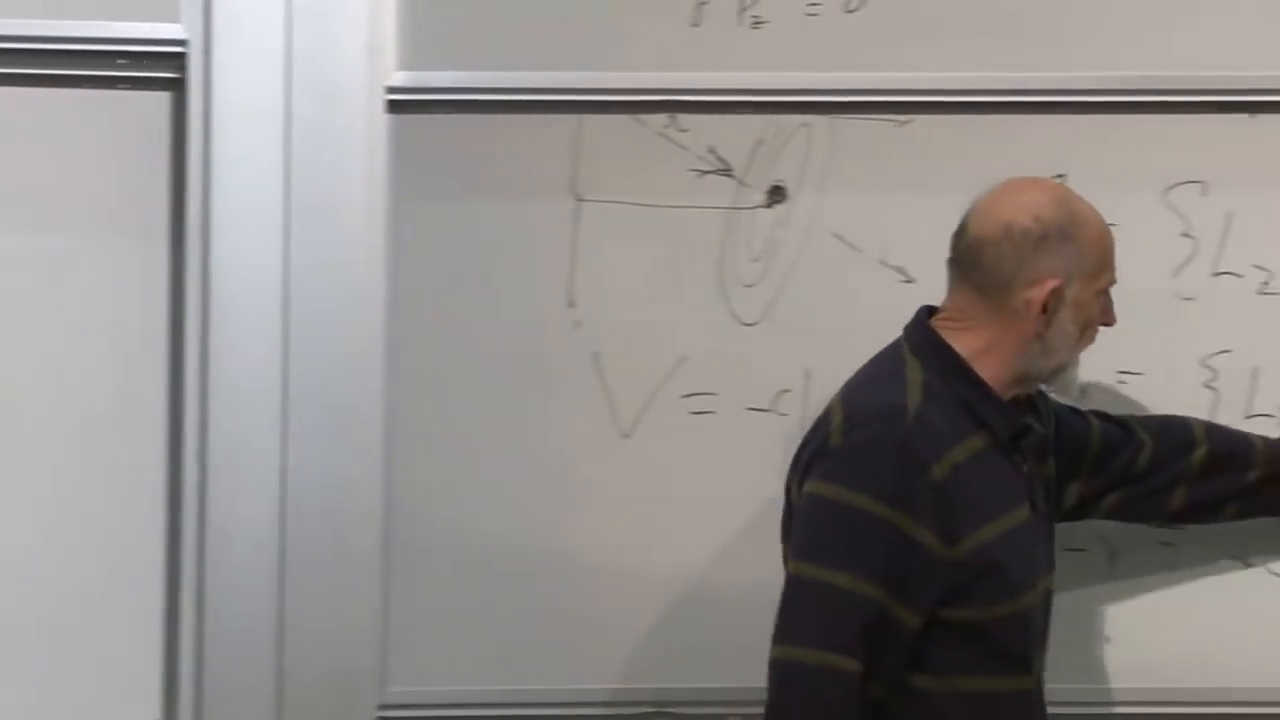
\includegraphics[width=0.82\textwidth]{lecture_08_figure_06.png}
  \caption{Los dos órdenes del mismo corchete nulo: conservación de \(G\) e invariancia de \(H\) bajo la transformación generada por \(G\).}
  \lectureframe{01:03:05}
\end{figure}

\begin{classroomqa}
  \audiencequestion{Si se conoce una cantidad conservada, ¿siempre se puede recuperar la simetría asociada? \lecturetimestamp{01:01:42--01:02:15}}
  \lecturerresponse{En este marco hamiltoniano, sí: se calcula el corchete de cada variable del espacio de fases con \(G\). El conjunto
  \(\delta_GA=\epsilon\{A,G\}\) indica cómo se transforman las variables. Por ejemplo, los corchetes con \(L_z\) revelan una rotación, aunque no se conociera de antemano esa interpretación. En marcos más avanzados pueden surgir sutilezas globales y de contorno, pero aquí se usa el enunciado infinitesimal local.}
\end{classroomqa}

\begin{classroomqa}
  \audiencequestion{¿Esas ecuaciones de corchetes nos dicen cuál es el movimiento físico responsable de la ley de conservación?
  \lecturetimestamp{00:56:01--00:58:13}}
  \lecturerresponse{No. Identifican la transformación de simetría, no la trayectoria real. La conservación de \(L_z\) indica simetría rotacional; no significa que la partícula se mueva en un círculo. La evolución temporal real está generada por \(H\). El corchete con otro generador describe otra dirección de transformación en el espacio de fases.}
\end{classroomqa}

\begin{classroomqa}
  \audiencequestion{¿Hay un enunciado general sobre las transformaciones que no presuponga ya la conservación? \lecturetimestamp{01:02:40--01:04:45}}
  \lecturerresponse{Sí. La ecuación~\eqref{eq:l8-generator-rule} define una transformación infinitesimal para cualquier función \(G\), se conserve o no. Solo se convierte en simetría cuando el hamiltoniano es invariante:
  \(\{H,G\}=0\). Leída en el orden inverso, la misma condición dice entonces que \(G\) se conserva.}
\end{classroomqa}

\section{El álgebra del momento angular}

El siguiente cálculo nos permitirá dejar de arrastrar las coordenadas de la partícula en cada problema de rotación. Empecemos con
\[
  L_x=yp_z-zp_y,\qquad
  L_z=xp_y-yp_x.
\]
En \(\{L_x,L_z\}\), la mayoría de los términos cruzados se anulan porque sus índices no forman pares canónicos. Las contracciones que sobreviven dan
\begin{align}
  \{L_x,L_z\}
  &=\{yp_z-zp_y,xp_y-yp_x\}\\
  &=xp_z-zp_x\\
  &=-L_y.
  \label{eq:l8-lx-lz}
\end{align}
Al invertir el orden, desaparece el signo menos. Al permutar cíclicamente las coordenadas se obtiene
\begin{equation}
  \boxed{\begin{aligned}
    \{L_x,L_y\}&=L_z,\\
    \{L_y,L_z\}&=L_x,\\
    \{L_z,L_x\}&=L_y.
  \end{aligned}}
  \label{eq:l8-angular-algebra}
\end{equation}
En notación de índices,
\begin{equation}
  \{L_i,L_j\}=\varepsilon_{ijk}L_k.
  \label{eq:l8-angular-algebra-index}
\end{equation}

\begin{figure}[htbp]
  \centering
  \includegraphics[width=0.82\textwidth]{lecture_08_figure_07.png}
  \caption{El álgebra cíclica de corchetes de Poisson de las tres componentes del momento angular.}
  \lectureframe{01:10:52}
\end{figure}

También se podría haber anticipado el resultado. Como \(\boldsymbol L\) es un vector, el corchete de su componente \(x\) con \(L_z\) debe dar el cambio infinitesimal de esa componente bajo una rotación alrededor del eje \(z\), es decir, \(-L_y\). El cálculo explícito confirma ese argumento geométrico. Estas ecuaciones son también precursoras clásicas de las relaciones de conmutación cuánticas del momento angular.

\section{Un giroscopio de giro rápido}

Como aplicación, consideremos un giroscopio: un volante que gira rápidamente y cuyo centro está a una distancia fija \(R\) de un pivote. Sea \(\boldsymbol r\) el vector que va del pivote al centro del volante. El volante gira tan rápidamente alrededor de su eje que el momento angular dominante permanece alineado con esa dirección. En la aproximación usada en la lección,
\begin{equation}
  \boldsymbol L=\ell\,\boldsymbol r,
  \qquad
  L_z=\ell z,
  \label{eq:l8-L-parallel-r}
\end{equation}
donde \(\ell=L/R\) se considera constante. En primera aproximación se desprecian los momentos angulares menores asociados a la nutación o al movimiento del eje.

\begin{figure}[htbp]
  \centering
  \begin{tikzpicture}[scale=0.95,>=Latex]
    \coordinate (P) at (0,3.2);
    \coordinate (C) at (3.7,1.55);
    \draw[->] (0,-0.2) -- (0,4.35) node[above] {\(z\)};
    \fill (P) circle (1.7pt) node[left] {pivot};
    \draw[very thick,->] (P) -- (C)
      node[midway,above right] {\(\boldsymbol r\parallel\boldsymbol L\)};
    \fill (C) circle (1.7pt);
    \draw[dashed] (P) -- (0,1.55);
    \draw[dashed] (0,1.55) -- (C);
    \node[left] at (0,1.55) {\(z\)};
    \begin{scope}[shift={(C)},rotate=-24]
      \draw[very thick] (0,0) ellipse (0.65 and 1.35);
      \draw[thick] (0,0) ellipse (0.42 and 0.9);
    \end{scope}
    \draw[->,thick] (2.15,2.85)
      arc[start angle=140,end angle=35,radius=1.65];
  \end{tikzpicture}
  \caption{Aproximación del giroscopio de giro rápido. La distancia del pivote al centro es fija y el momento angular dominante del giro permanece alineado con el eje y con \(\boldsymbol r\).}
\end{figure}

\begin{figure}[htbp]
  \centering
  \includegraphics[width=0.82\textwidth]{lecture_08_figure_08.png}
  \caption{El esquema de la pizarra del volante, junto con \(H_{\rm rot}=L^2/(2I)\) y la cancelación que demuestra la conservación de \(\boldsymbol L\) cuando no hay torque.}
  \lectureframe{01:18:54}
\end{figure}

\subsection{Sin gravedad: por qué permanece fija cada componente}

Para el rotor axialsimétrico simplificado,
\begin{equation}
  H_{\mathrm{rot}}
  =\frac{1}{2I}
  \left(L_x^2+L_y^2+L_z^2\right)
  =\frac{L^2}{2I}.
  \label{eq:l8-rotational-hamiltonian}
\end{equation}
El coeficiente es \(1/(2I)\), no \(I/2\); ese desliz se comete y se corrige en la pizarra. Usando la ec.~\eqref{eq:l8-angular-algebra},
\begin{align}
  \dot L_x
  &=\{L_x,H_{\mathrm{rot}}\}\\
  &=\frac{1}{2I}\left(
    2L_y\{L_x,L_y\}
    +2L_z\{L_x,L_z\}
  \right)\\
  &=\frac{1}{I}\left(L_yL_z-L_zL_y\right)=0.
  \label{eq:l8-free-lx}
\end{align}
Y cíclicamente,
\begin{equation}
  \dot L_x=\dot L_y=\dot L_z=0.
  \label{eq:l8-free-angular-momentum}
\end{equation}
El escalar \(L^2\) tiene corchete nulo con cada componente \(L_i\); en el lenguaje de esta álgebra, es un casimir. Así, un giroscopio sin torque conserva tanto el módulo como la dirección de su momento angular.

\begin{classroomqa}
  \audiencequestion{¿El momento de inercia es simplemente un número aquí?
  \lecturetimestamp{01:14:23--01:15:05}}
  \lecturerresponse{Sí, para este modelo reducido. Representa la distribución de masa del volante respecto de su eje de giro. Un cuerpo rígido general tiene un tensor de momento de inercia y un hamiltoniano rotacional
  \(\sum_i L_i^2/(2I_i)\) en los ejes principales. La lección elige el rotor simétrico de giro rápido, más sencillo, porque el objetivo es mostrar el método de los corchetes de Poisson, no desarrollar la dinámica completa de los cuerpos rígidos.}
\end{classroomqa}

\subsection{La gravedad y el signo del potencial}

Tomemos la coordenada vertical \(z\) positiva hacia arriba y situemos el pivote en el origen. La energía potencial gravitatoria del centro del volante es
\begin{equation}
  V=Mgz.
  \label{eq:l8-mgz}
\end{equation}
Como \(L_z=\ell z\),
\begin{equation}
  V=cL_z,
  \qquad
  c=\frac{Mg}{\ell}=\frac{MgR}{L}.
  \label{eq:l8-potential-lz}
\end{equation}
Aquí \(c>0\) cuando se elige \(\boldsymbol L\) paralelo a \(\boldsymbol r\). Si el volante gira en el sentido opuesto, se invierte la relación con signo entre \(\boldsymbol L\) y \(\boldsymbol r\), y también la frecuencia de precesión con su signo correspondiente.

\begin{figure}[htbp]
  \centering
  \includegraphics[width=0.82\textwidth]{lecture_08_figure_09.png}
  \caption{La geometría de longitud fija que subyace a \(\boldsymbol L=\ell\boldsymbol r\) y \(L_z=\ell z\).}
  \lectureframe{01:25:38}
\end{figure}

\begin{figure}[htbp]
  \centering
  \includegraphics[width=0.82\textwidth]{lecture_08_figure_10.png}
  \caption{Un estado intermedio de la pizarra muestra \(V=-cL_z\). El signo se corrige más adelante, una vez que \(z\) se fija hacia arriba: con \(\boldsymbol L=\ell\boldsymbol r\) y \(\ell>0\), el resultado coherente es \(V=+cL_z\).}
  \lectureframe{01:22:43}
\end{figure}

\begin{classroomqa}
  \audiencequestion{¿Por qué se puede sustituir la altura por una componente del momento angular? ¿La línea inclinada representa un eje o un vector de posición?
  \lecturetimestamp{01:22:20--01:25:43}}
  \lecturerresponse{Conviene etiquetar la línea inclinada como \(\boldsymbol r\), el vector que va del pivote fijo al centro del volante. Un eje físico puede estar alineado con ella, pero la relación usada en el cálculo es la aproximación de giro rápido
  \(\boldsymbol L=\ell\boldsymbol r\). Por tanto, sus componentes \(z\) son proporcionales. En la explicación en vivo se cambian las etiquetas varias veces antes de establecer esta distinción.}
\end{classroomqa}

\begin{classroomqa}
  \audiencequestion{¿Qué supuestos hacen que \(\ell\) sea constante, y qué falla si el centro del volante puede deslizarse radialmente?
  \lecturetimestamp{01:25:43--01:26:38,\allowbreak\ 01:34:22--01:35:00}}
  \lecturerresponse{Se supone que el giro dominante es mucho mayor que el momento angular asociado al movimiento lento y que la distancia del pivote al centro es fija. Entonces, el módulo del giro apenas cambia y \(\boldsymbol L\) rota junto con \(\boldsymbol r\). Si el centro pudiera deslizarse radialmente, \(z\) dejaría de ser proporcional a \(L_z\) con un único coeficiente constante, por lo que el hamiltoniano reducido \(V=cL_z\) ya no describiría el movimiento.}
\end{classroomqa}

\begin{classroomqa}
  \audiencequestion{¿Por qué la pizarra muestra primero un signo menos y luego uno más? ¿Importa el sentido del giro?
  \lecturetimestamp{01:27:13--01:28:15,\allowbreak\ 01:33:09--01:33:21}}
  \lecturerresponse{El signo inicial es un error de pizarra cometido en vivo, mezclado con una convención de ejes aún sin fijar. Una vez que \(z\) se define hacia arriba, \(V=Mgz\) aumenta con la altura. Si \(\boldsymbol L=\ell\boldsymbol r\) con \(\ell>0\), resulta \(V=+cL_z\). Invertir el sentido del giro invierte la proporcionalidad con signo y el sentido de la precesión, pero no permite elegir arbitrariamente el signo.}
\end{classroomqa}

\subsection{La precesión en tres ecuaciones breves}

El hamiltoniano reducido completo es
\begin{equation}
  H=
  \frac{1}{2I}\left(L_x^2+L_y^2+L_z^2\right)+cL_z.
  \label{eq:l8-full-gyro-hamiltonian}
\end{equation}
Ya hemos demostrado que \(L^2\) tiene corchete nulo con cada \(L_i\). Solo contribuye el término lineal:
\begin{align}
  \dot L_z&=\{L_z,H\}=0,\\
  \dot L_x&=\{L_x,H\}=c\{L_x,L_z\}=-cL_y,\\
  \dot L_y&=\{L_y,H\}=c\{L_y,L_z\}=cL_x.
  \label{eq:l8-precession-equations}
\end{align}

\begin{figure}[htbp]
  \centering
  \includegraphics[width=0.82\textwidth]{lecture_08_figure_11.png}
  \caption{Las ecuaciones finales para las componentes: \(L_z\) es constante, mientras que \(L_x\) y \(L_y\) rotan una en la otra.}
  \lectureframe{01:30:35}
\end{figure}

La componente vertical y el módulo de la componente horizontal son constantes:
\begin{equation}
  \frac{d}{dt}(L_x^2+L_y^2)
  =2L_x(-cL_y)+2L_y(cL_x)=0.
\end{equation}
Al combinar las componentes horizontales,
\begin{equation}
  L_+=L_x+iL_y,
  \qquad
  \dot L_+=icL_+,
\end{equation}
se obtiene
\begin{equation}
  L_+(t)=L_+(0)e^{ict}.
  \label{eq:l8-precession-solution}
\end{equation}
Por tanto, el vector de momento angular precesa alrededor del eje vertical con rapidez angular \(|c|=MgR/L\). En este movimiento estacionario idealizado, su inclinación permanece fija.

\begin{classroomqa}
  \audiencequestion{¿Se omitió el término de energía rotacional al escribir las ecuaciones de precesión?
  \lecturetimestamp{01:35:01--01:35:49}}
  \lecturerresponse{No. Forma parte del hamiltoniano completo, como en la ec.~\eqref{eq:l8-full-gyro-hamiltonian}. Simplemente aporta cero a \(\dot L_i\) porque \(\{L_i,L^2\}=0\), una cancelación ya demostrada en el cálculo sin torque. La pregunta del estudiante hace explícito este paso implícito.}
\end{classroomqa}

\begin{classroomqa}
  \audiencequestion{¿La precesión uniforme es un equilibrio? ¿Qué ocurre después de un pequeño impulso? \lecturetimestamp{01:32:38--01:33:08}}
  \lecturerresponse{Es más apropiado llamarla movimiento estacionario que equilibrio estático. Un pequeño impulso suele añadir nutación, es decir, una oscilación del ángulo de inclinación. En un volante de giro muy rápido, esa oscilación es pequeña; por eso el tratamiento reducido solo considera una precesión casi uniforme.}
\end{classroomqa}

\begin{classroomqa}
  \audiencequestion{¿La precesión requiere un soporte o un eje físico?
  \lecturetimestamp{01:31:49--01:32:38,\allowbreak\ 01:33:49--01:35:00}}
  \lecturerresponse{Este modelo mecánico supone fija la distancia del pivote al centro, así que alguna ligadura proporciona el soporte. El resultado algebraico más profundo es más general: siempre que el hamiltoniano contenga un término lineal en una componente del momento angular, la misma álgebra de corchetes produce precesión. El origen microscópico del momento angular no tiene por qué ser una rueda real montada sobre un eje.}
\end{classroomqa}

\begin{classroomqa}
  \audiencequestion{¿Es esta la misma precesión que la del espín electrónico o nuclear en un campo magnético, o que la precesión de la órbita de un planeta?
  \lecturetimestamp{01:35:50--01:37:00}}
  \lecturerresponse{Un momento magnético acoplado a un campo magnético tiene un hamiltoniano lineal en una componente del espín y, por tanto, obedece la misma álgebra del momento angular. La precesión del espín nuclear es la base de la resonancia magnética nuclear. La precesión del perihelio de una órbita planetaria es un fenómeno distinto que comparte la palabra \emph{precesión}; no se obtiene mediante el mismo cálculo.}
\end{classroomqa}

\begin{classroomqa}
  \audiencequestion{¿Es esencialmente el mismo objeto el giroscopio montado lateralmente que una peonza? \lecturetimestamp{01:37:02--01:37:23}}
  \lecturerresponse{Sí. La diferencia es principalmente geométrica y terminológica: cuando el eje de giro sobresale lateralmente del soporte, suele hablarse de giroscopio; cuando está casi vertical, se habla de peonza. La estructura del momento angular y del torque es la misma.}
\end{classroomqa}

\section{Qué se logró con el cálculo}

No se introdujeron ángulos de Euler ni se siguieron las coordenadas de cada parte de la rueda. Una vez conocida
\[
  \{L_i,L_j\}=\varepsilon_{ijk}L_k
\]
las ecuaciones de las variables de interés se obtuvieron directamente. Esa es la demostración de potencia que se busca. El oscilador mostró que los corchetes de Poisson pueden reproducir dinámicas conocidas. El momento angular mostró que sirven para mucho más:
\begin{itemize}
  \item una cantidad conservada genera su simetría infinitesimal asociada;
  \item la conservación de \(G\) y la invariancia de \(H\) son las dos interpretaciones de \(\{G,H\}=0\);
  \item el álgebra de los observables puede cerrarse sobre sí misma, lo que permite resolver la dinámica sin volver a las coordenadas microscópicas;
  \item un hamiltoniano lineal en una componente del momento angular produce precesión alrededor de ese eje.
\end{itemize}
La lección termina antes de abordar las ecuaciones de Euler completas para un cuerpo rígido general. Su conclusión más acotada ya está completa: los generadores adecuados y su álgebra de Poisson ponen de manifiesto tanto la simetría como el movimiento con notable economía.
